\chapter{Движение по окружности. Передачи.}
{\bfseries Анонс:}\\\\
Характеристики движения по окружности: скорость, период, частота, угловая скорость. Виды передач: фрикционная, ременная, зубчатая, червячная.\\\\
{\bfseries Цели:}
\begin{itemize}
	\item{}{\bfseries Обучающие:} Познакомить с основными понятиями кинематики криволинейного движения. Сформировать у учащихся представления об основных видах механических передач.
	\item{}{\bfseries Развивающие:}Формирование умений сравнивать, классифицировать, обобщать изучаемые факты и понятия. Развитие познавательного интереса для учащихся.\\
\end{itemize}	
{\bfseries Ход занятия:}\\\\
\begin{tabular}{lll}
	\hyperlink{lesson5x1}{1. Организационный момент} & Презентация & (5 мин)\\
	\hyperlink{lesson5x2}{2. Характеристики движения} & Презентация & (50 мин) \\
	\hyperlink{lesson5x3}{3. Виды передач} & Презентация & (20 мин) \\
	\hyperlink{lesson5x4}{4. Решение задач} & Практика & (30 мин)\\
\end{tabular}\\\\

{\hypertarget{lesson5x1}{\blackBlueText{I.Организационный момент}}}\\\\

В первой половине занятия предполагается запись теории и решение задач, поэтому следует заранее предупредить учащихся о необходимости принести тетради/блокноты. Рассказ по видам механических передач рекомендуется дополнять демонстрациями этих передач на макетах и видео.

Во второй части занятия следует решить несколько задач на характеристики движения по окружности.\\\\

{\hypertarget{lesson5x2}{\blackBlueText{II. Характеристики движения}}}\\\\

{\slshape Курс рассчитан на учащихся 8-ого класса и старше, так что при дальнейшем изложении материала предполагаются известными характеристики путь и скорость.} 

При движении тела по окружности (вращении)  зачастую оказывается удобно говорить не о пути s, пройденным телом, а об угле поворота \(\phi\). Угол \(\phi\) принято измерять не в градусах, а в специальных единицах радианах (рад). По определению радиана:
\begin{equation}
\phi=\frac{s}{r}
\end{equation}
\begin{figure}[h!]
	\begin{center}
		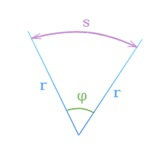
\includegraphics[width=0.27\linewidth]{chapters/chapter5/images/1}
		\caption{}
		\label{ris:image5x0x1}
	\end{center}
\end{figure}

Тогда получается, что вся окружность имеет угловую меру:
\begin{equation}
\phi=\frac{s}{r}=\frac{2\pi r}{r}=2\pi\mbox{ \slshape рад}
\end{equation}

С другой стороны, вся окружность имеет градусную меру \(360^{\circ}\). Таким образом, получаем формулу для перевода градусов в радианы и наоборот:
\begin{equation}
\frac{\phi_{\mbox{ \slshape рад}}}{\phi^{\circ}}=\frac{\pi}{180^{\circ}}
\end{equation}

Время одного полного оборота называют периодом и обозначают буквой \(T\). Величина, обратная периоду носит название частота, и обозначается буквой \(\nu\). Частота измеряется в герцах (Гц) и имеет смысл числа оборотов за единицу времени.
\begin{equation}
[T]=\mbox{\slshape c}
\end{equation} 
\begin{equation}
[\nu]=\frac{1}{\mbox{\slshape c}}=\mbox{\slshape Гц}
\end{equation}  
\begin{equation}
{T=\frac{1}{\nu}}
\end{equation}

При движении по окружности различают линейную и угловую скорости. Линейная скорость \(V\)~--- это путь \(\Delta s\), проходимый за единицу времени, так сказать «обычная» скорость. Угловой скоростью \(\omega\) называют угол \(\Delta\phi\), на который повернулось тело за единицу времени. Легко вывести формулу, связывающую линейную и угловую скорости.
\begin{equation}
V=\frac{\Delta s}{\Delta t}
\end{equation}
\begin{equation}
\omega=\frac{\Delta\phi}{\Delta t}
\end{equation} 
\begin{equation}
V=\frac{\Delta s}{\Delta t}=\frac{\Delta (\phi r)}{\Delta t}=\frac{r\Delta\phi}{\Delta t}=\omega r
\end{equation} 

За один полный оборот тело поворачивается на угол \(2\pi\) радиан, затрачивая на это время равное периоду \(T\). Тогда угловая скорость:
\begin{equation}
\omega=\frac{2\pi}{T}=2\pi\nu
\end{equation}\\\\

{\hypertarget{lesson5x3}{\blackBlueText{III. Виды передач}}}\\\\

При построении сложных механизмов часто возникает необходимость передавать вращение от мотора к другим частям конструкции. Для этого применяют различные виды передач: фрикционные, зубчатые, ременные, цепные и червячные.
\begin{figure}[h!]
	\begin{center}
		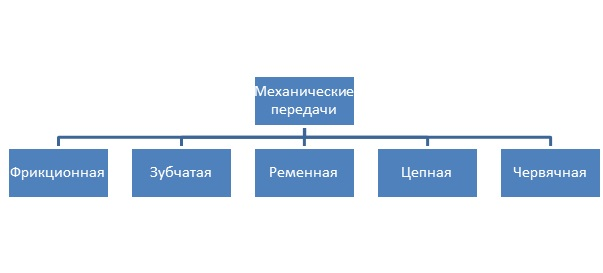
\includegraphics[width=0.9\linewidth]{chapters/chapter5/images/2}
		\caption{}
		\label{ris:image5x1}
	\end{center}
\end{figure}

При {\bfseries фрикционной} передаче вращение от одного колеса к другому передается при помощи силы трения. Оба колеса прижимаются друг к другу с некоторой силой и вследствие возникающего между ними трения вращают одно другое.\\
Достоинства фрикционной передачи:

\begin{itemize}
	\item Простота изготовления тел качения;	
	\item Равномерность вращения и бесшумность работы;
	\item Возможность включения/выключения передачи на ходу.\\
\end{itemize}
Недостатки фрикционной передачи:

\begin{itemize}
	\item Проскальзывание, ведущее к непостоянству передаточного числа и потери энергии;
	
	\item Необходимость обеспечения прижима.\\\\
\end{itemize}
\begin{figure}[h!]
	\begin{center}
		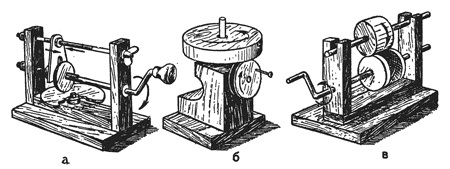
\includegraphics[width=1\linewidth]{chapters/chapter5/images/3}
		\caption{а~--- лобовая передача, б~--- угловая передача, в~--- цилиндрическая передача.}
		\label{ris:image5x2}
	\end{center}
\end{figure}
\clearpage
\begin{figure}[h!]
	\begin{center}
		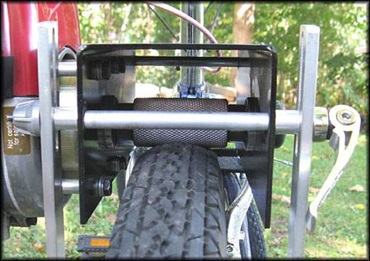
\includegraphics[width=1\linewidth]{chapters/chapter5/images/4}
		\caption{}
		\label{ris:image5x3}
	\end{center}
\end{figure}
\clearpage
В {\bfseries зубчатых} передачах вращение от одного колеса к другому передается при помощи зубьев. Зубчатые колеса вращаются намного легче фрикционных. Объясняется это тем, что здесь нажима колеса на колесо совсем не требуется. Для правильного зацепления и легкой работы колес профиль зубца делают по определенной кривой, называемой эвольвентой.
\begin{figure}[h!]
	\begin{center}
		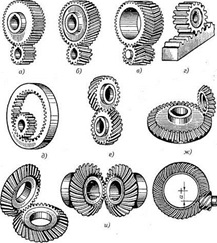
\includegraphics[width=1\linewidth]{chapters/chapter5/images/5}
		\caption{}
		\label{ris:image5x4}
	\end{center}
\end{figure}
\clearpage
\begin{figure}[h!]
	\begin{center}
		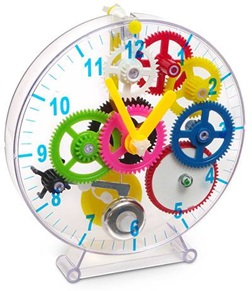
\includegraphics[width=1\linewidth]{chapters/chapter5/images/6}
		\caption{}
		\label{ris:image5x5}
	\end{center}
\end{figure}
Достоинства зубчатой передачи:

\begin{itemize}
	\item Значительно меньшие габариты, чем у других передач;	
	\item Высокий кпд (потери в точных, хорошо смазываемых передачах 1--2\%);	
	\item Большая долговечность и надёжность.\\
\end{itemize}
Недостатки зубчатой передачи:

\begin{itemize}
	\item Шум при работе;	
	\item Необходимость точного изготовления.\\
\end{itemize}

{\bfseries Ременная} передача, как и зубчатая, встречается очень часто. Ремень, натянутый на шкивы, охватывает какую-то их часть. Эта облегающая часть (дуга) носит, название угла обхвата. Чем больше будет угол обхвата, тем лучше образуется сцепление, лучше и надежнее будет вращение шкивов. При малом угле обхвата может получиться так, что ремень на малом шкиве станет проскальзывать, вращение будет передаваться плохо или его совсем не будет. Угол обхвата зависит от соотношения размеров шкивов и их расстояния друг от друга.

\begin{figure}[h!]
	\begin{center}
		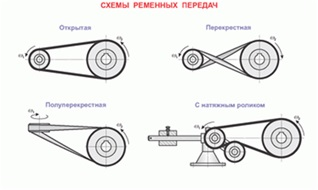
\includegraphics[width=0.55\linewidth]{chapters/chapter5/images/7}
		\caption{Схемы ременчатых передач.}
		\label{ris:image5x6}
	\end{center}
\end{figure}
\begin{figure}[h!]
	\begin{center}
		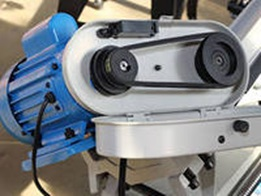
\includegraphics[width=0.55\linewidth]{chapters/chapter5/images/8}
		\caption{Схемы ременчатых передач.}
		\label{ris:image5x7}
	\end{center}
\end{figure}
\clearpage
\noindent Достоинства ременной передачи:	

\begin{itemize}
	\item Простота конструкции;
	\item Возможность расположения ведущего и ведомого шкивов на больших расстояниях (более 15 метров);
	\item Плавность и бесшумность работы;
	\item Предохранение механизмов от перегрузки за счёт упругих свойств ремня и его способности проскальзывать по шкивам;
	\item Возможность работы с большими угловыми скоростями.\\
\end{itemize}
\noindent Недостатки ременной передачи:

\begin{itemize}
	\item Постепенное вытягивание ремней, их недолговечность (при больших скоростях работает от 1000 до 5000 часов);
	\item Непостоянство передаточного отношения (из-за неизбежного проскальзывания ремня);
	\item Относительно большие размеры.\\
\end{itemize}

{\bfseries Цепная} передача по сравнению с ременной удобна тем, что не дает проскальзывания и позволяет соблюдать правильность передаточного числа. Цепная передача осуществляется только при параллельных валах.

\begin{figure}[h!]
	\begin{center}
		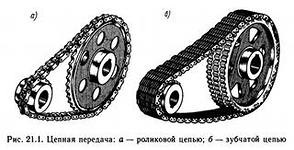
\includegraphics[width=1\linewidth]{chapters/chapter5/images/9}
		\caption{}
		\label{ris:image5x8}
	\end{center}
\end{figure}	
\clearpage
\begin{figure}[h!]
	\begin{center}
		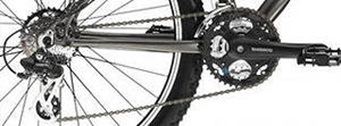
\includegraphics[width=0.72\linewidth]{chapters/chapter5/images/10}
		\caption{}
		\label{ris:image5x9}
	\end{center}
\end{figure}	
\noindent Достоинства цепной передачи:	

\begin{itemize}
	\item Меньшая чувствительность к неточностям расположения валов;
	\item Возможность передачи движения одной цепью нескольким звездочкам;
	\item Возможность передачи вращательного движения на большие расстояния.\\
\end{itemize}
Недостатки цепной передачи:

\begin{itemize}
	\item Повышенный шум и износ цепи при неправильном выборе конструкции, небрежном монтаже и плохом уходе.\\
\end{itemize}

{\bfseries Червячная} передача служит для получения вращения между валами, пересекающимися в одной плоскости. Передача состоит из винта (червяка) и винтового колеса, которые находятся в зацеплении. При вращении червяка витки ведут зубцы колеса и заставляют его вращаться. Обычно вращение от червяка передается колесу. Обратная передача почти не встречается из-за самоторможения.

\begin{figure}[h!]
	\begin{center}
		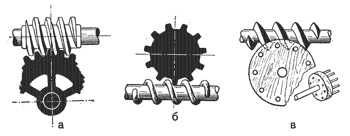
\includegraphics[width=0.8\linewidth]{chapters/chapter5/images/11}
		\caption{}
		\label{ris:image5x10}
	\end{center}
\end{figure}
\clearpage
\begin{figure}[h!]
	\begin{center}
		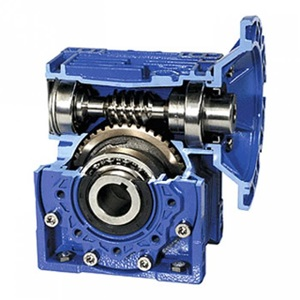
\includegraphics[width=0.90\linewidth]{chapters/chapter5/images/12}
		\caption{Схемы ременчатых передач.}
		\label{ris:image5x11}
	\end{center}
\end{figure}	
\noindent Достоинства червячной передачи:	

\begin{itemize}
	\item Плавность и бесшумность работы;
	\item Большое передаточное число;
	\item Передача вращения только в одном направлении.\\
\end{itemize}
Недостатки червячной передачи:

\begin{itemize}
	\item Усиленное тепловыделение;
	\item Повышенный износ;
	\item Склонность к заеданию;
	\item Сравнительно низкий кпд.\\\\
\end{itemize}

{\hypertarget{lesson5x4}{\blackBlueText{IV. Решение задач}}}\\\\

Теоретический материал из предыдущих пунктов рекомендуется дополнить решением задач. Часть из них может быть разобрана в классе, часть дана для самостоятельного изучения.

В зависимости от конкретной ситуации, учащихся можно вызывать на задачу «змейкой», каждый делает ровно одно действие; либо можно устроить небольшой турнир по задачам или «свою игру», с «котом в мешке» (например, построить реальную фрикционную передачу из стирательных резинок) и «вопросом-аукцион».\\\\

\newcounter{tasks}
\begin{itemize}
	\renewcommand{\labelitemi}{\stepcounter{tasks}\Roman{tasks}.}
	%\renewcommand{\theenumi}{\Roman{enumi}}
	\item Частота обращения ветроколеса ветродвигателя 30 об/мин, якоря электродвигателя 1500 об/мин, барабана сепаратора 8400 об/мин, шпинделя шлифовального станка 96 000 об/мин. Вычислить их периоды.
	\item Скорость точек рабочей поверхности наждачного круга диаметром 300 мм не должна превышать 35 м/с. Допустима ли посадка круга на вал электродвигателя, совершающего 1400 об/мин; 2800 об/мин?
	\item Частота обращения воздушного винта самолета 1500 об/мин. Сколько оборотов делает винт на пути 90 км при скорости полета 180 км/ч?
	\item Период обращения платформы карусельного станка 4 с. Найти скорость крайних точек платформы, удаленных от оси вращения на 2 м.
	\item Диаметр передних колес трактора в 2 раза меньше, чем задних. Сравнить частоты обращения колес при движении трактора.
	\item Радиус рукоятки колодезного ворота в 3 раза больше радиуса вала, на который наматывается трос. Какова линейная скорость конца рукоятки при поднятии ведра с глубины 10 м за 20 с?
	\item При увеличении в 4 раза радиуса круговой орбиты искусственного спутника Земли период его обращения увеличивается в 8 раз. Во сколько раз изменяется скорость движения спутника по орбите?	
	\item Минутная стрелка часов в 3 раза длиннее секундной. Найти отношение скоростей концов стрелок.\\
\end{itemize}